\documentclass[11pt]{article}
\usepackage[textwidth=18.0cm, textheight=23.0cm, top=2.0cm]{geometry}
\usepackage{pst-all}
\usepackage{amssymb}
\usepackage{tikz}
\usepackage{underscore}\begin{document}
\pagestyle{empty}


ClassName: \underline{\textbf{Class_07.2bp-19}}
\par
BinSize: \underline{\textbf{100 × 100}}
\par
ReduceSize: \underline{\textbf{100 × 100}}
\par
TypeNum: \underline{\textbf{39}}
\par
Num: \underline{\textbf{40}}
\par
OutS: \underline{\textbf{130000}}
\par
InS: \underline{\textbf{102031}}
\par
Rate: \underline{\textbf{0.785}}
\par
UB: \underline{\textbf{13}}
\par
LB0: \underline{\textbf{13}}
\par
LB: \underline{\textbf{13}}
\par
LBWithCut: \underline{\textbf{13}}
\par
NodeCut: \underline{\textbf{0}}
\par
ExtendedNodeCnt: \underline{\textbf{1}}
\par
GenNodeCnt: \underline{\textbf{1}}
\par
PrimalNode: \underline{\textbf{0}}
\par
ColumnCount: \underline{\textbf{13}}
\par
TotalCutCount: \underline{\textbf{0}}
\par
RootCutCount: \underline{\textbf{0}}
\par
LPSolverCnt: \underline{\textbf{1}}
\par
PricingSolverCnt: \underline{\textbf{0}}
\par
BranchAndBoundNum: \underline{\textbf{1}}
\par
isOpt: \underline{\textbf{true}}
\par
TimeOnPrimal: \underline{\textbf{0.000 s}}
\par
TimeOnPricing: \underline{\textbf{0.000 s}}
\par
TimeOnRmp: \underline{\textbf{0.079 s}}
\par
TotalTime: \underline{\textbf{0.125 s}}
\par
\newpage


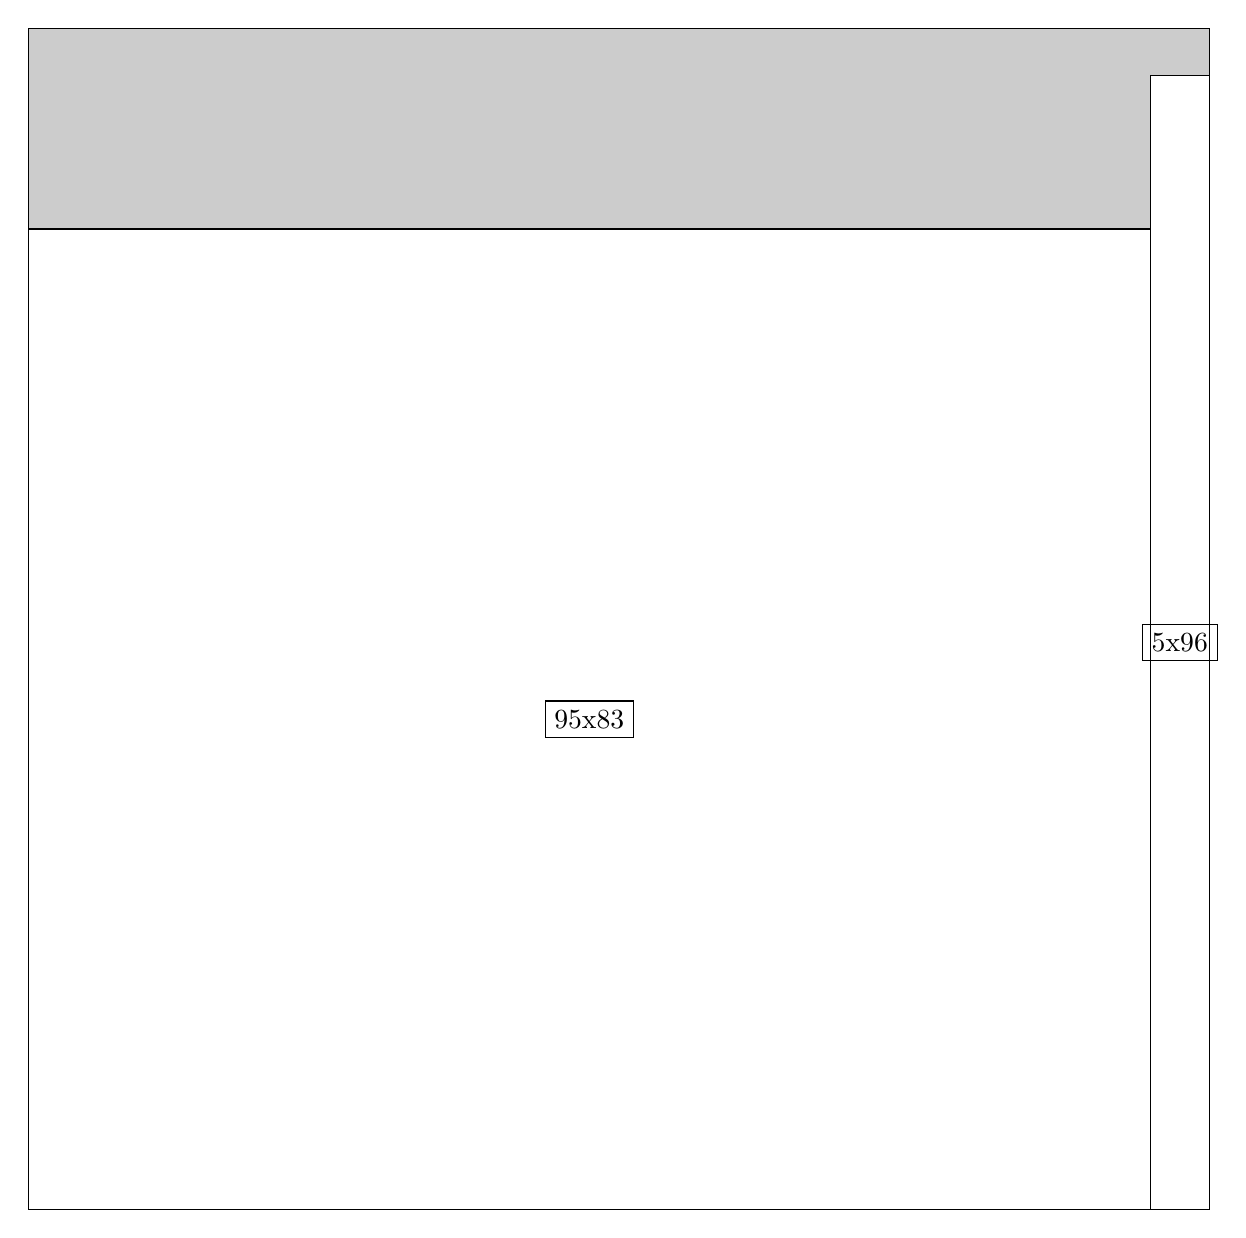
\begin{tikzpicture}[shorten >=1pt,scale=1.0,every node/.style={scale=1.0},->]
\tikzstyle{vertex}=[circle,fill=black!25,minimum size=14pt,inner sep=0pt]
\filldraw[fill=gray!40!white, draw=black] (0,0) rectangle (15.0,15.0);
\foreach \name/\x/\y/\w/\h in {95x83/0.0/0.0/14.25/12.45,5x96/14.25/0.0/0.75/14.399999999999999}
\filldraw[fill=white!40!white, draw=black] (\x,\y) rectangle node[draw] (\name) {\name} ++(\w,\h);
\end{tikzpicture}


w =95 , h =83 , x =0 , y =0 , v =7885
\par
w =5 , h =96 , x =95 , y =0 , v =480
\par
\newpage


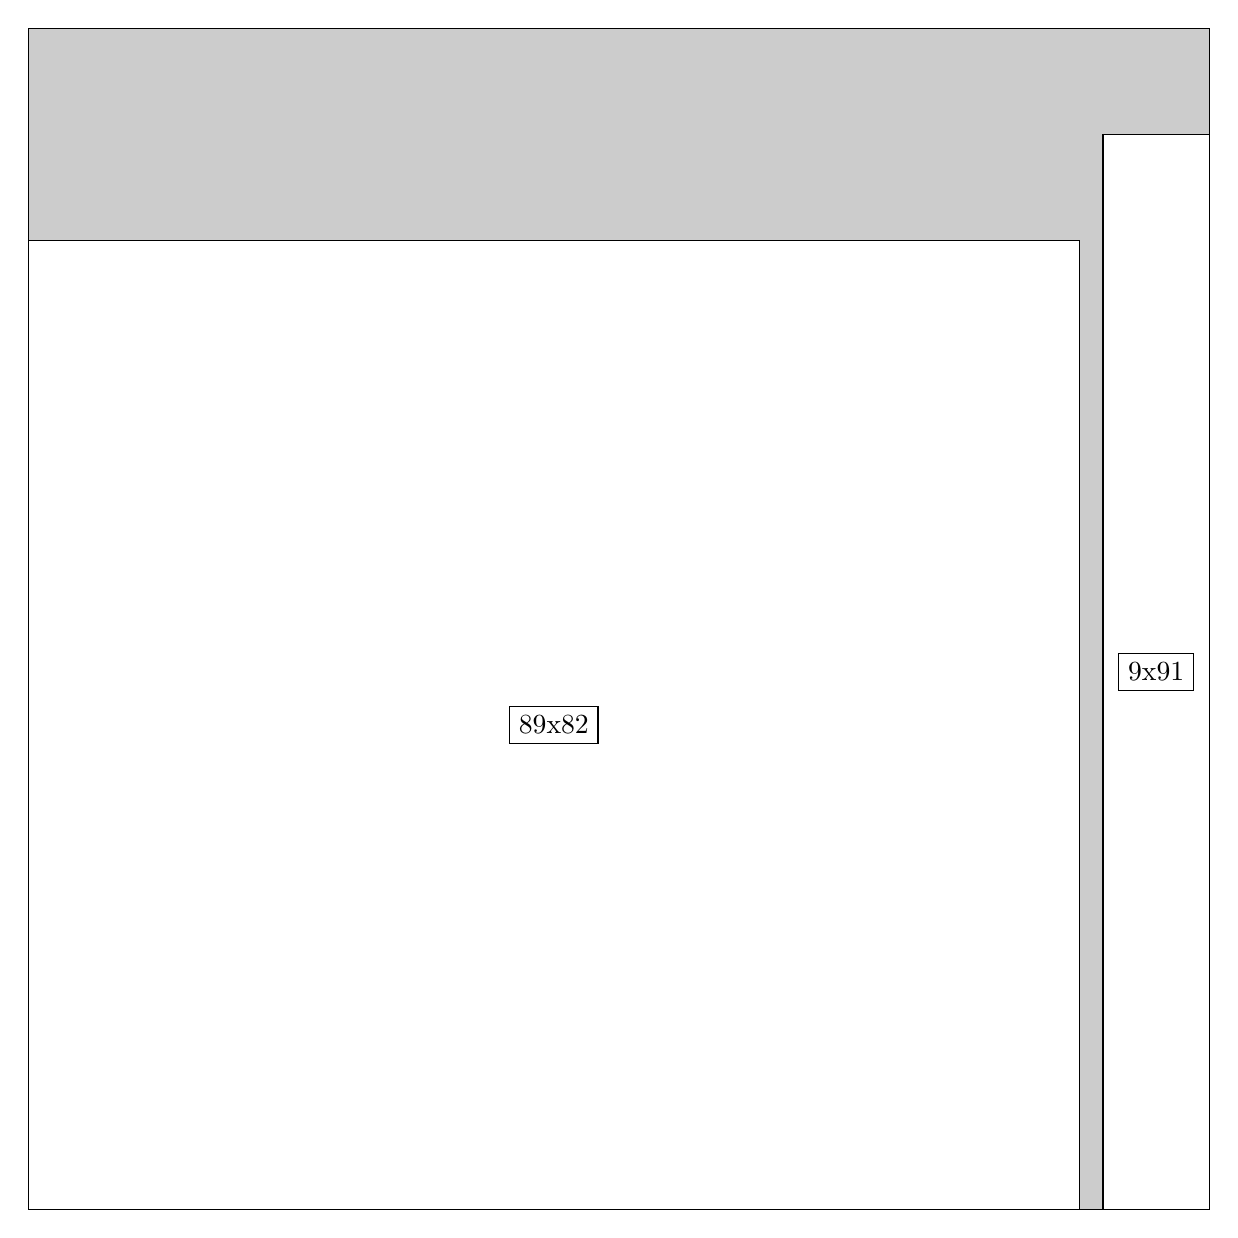
\begin{tikzpicture}[shorten >=1pt,scale=1.0,every node/.style={scale=1.0},->]
\tikzstyle{vertex}=[circle,fill=black!25,minimum size=14pt,inner sep=0pt]
\filldraw[fill=gray!40!white, draw=black] (0,0) rectangle (15.0,15.0);
\foreach \name/\x/\y/\w/\h in {89x82/0.0/0.0/13.35/12.299999999999999,9x91/13.65/0.0/1.3499999999999999/13.65}
\filldraw[fill=white!40!white, draw=black] (\x,\y) rectangle node[draw] (\name) {\name} ++(\w,\h);
\end{tikzpicture}


w =89 , h =82 , x =0 , y =0 , v =7298
\par
w =9 , h =91 , x =91 , y =0 , v =819
\par
\newpage


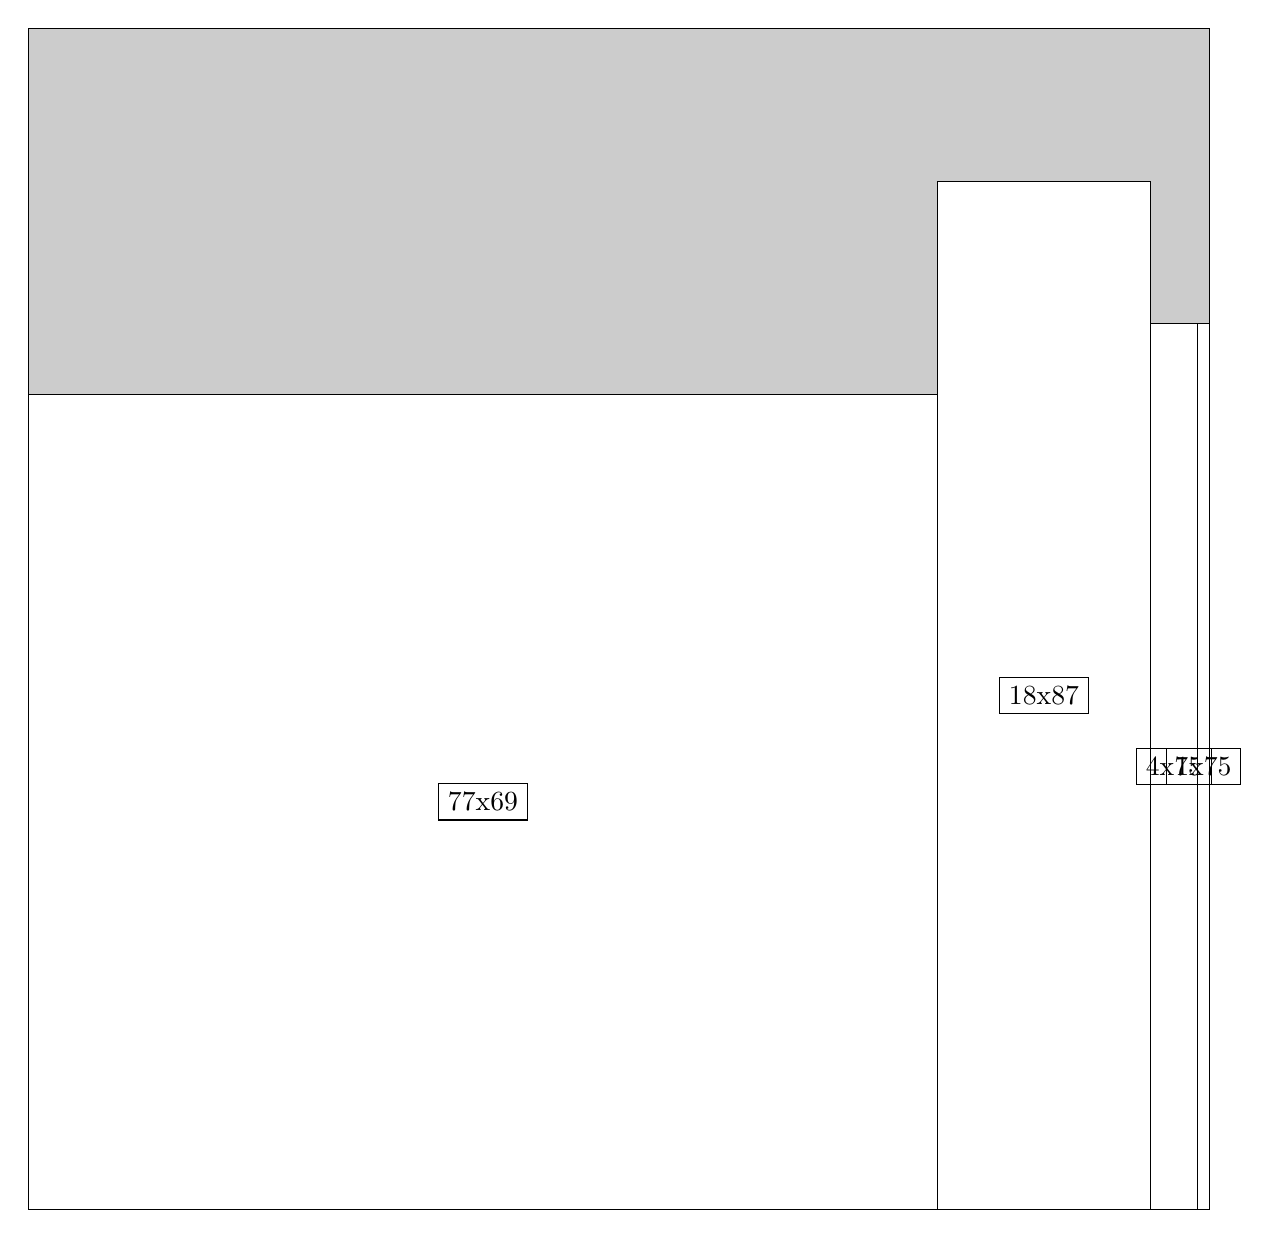
\begin{tikzpicture}[shorten >=1pt,scale=1.0,every node/.style={scale=1.0},->]
\tikzstyle{vertex}=[circle,fill=black!25,minimum size=14pt,inner sep=0pt]
\filldraw[fill=gray!40!white, draw=black] (0,0) rectangle (15.0,15.0);
\foreach \name/\x/\y/\w/\h in {77x69/0.0/0.0/11.549999999999999/10.35,18x87/11.549999999999999/0.0/2.6999999999999997/13.049999999999999,4x75/14.25/0.0/0.6/11.25,1x75/14.85/0.0/0.15/11.25}
\filldraw[fill=white!40!white, draw=black] (\x,\y) rectangle node[draw] (\name) {\name} ++(\w,\h);
\end{tikzpicture}


w =77 , h =69 , x =0 , y =0 , v =5313
\par
w =18 , h =87 , x =77 , y =0 , v =1566
\par
w =4 , h =75 , x =95 , y =0 , v =300
\par
w =1 , h =75 , x =99 , y =0 , v =75
\par
\newpage


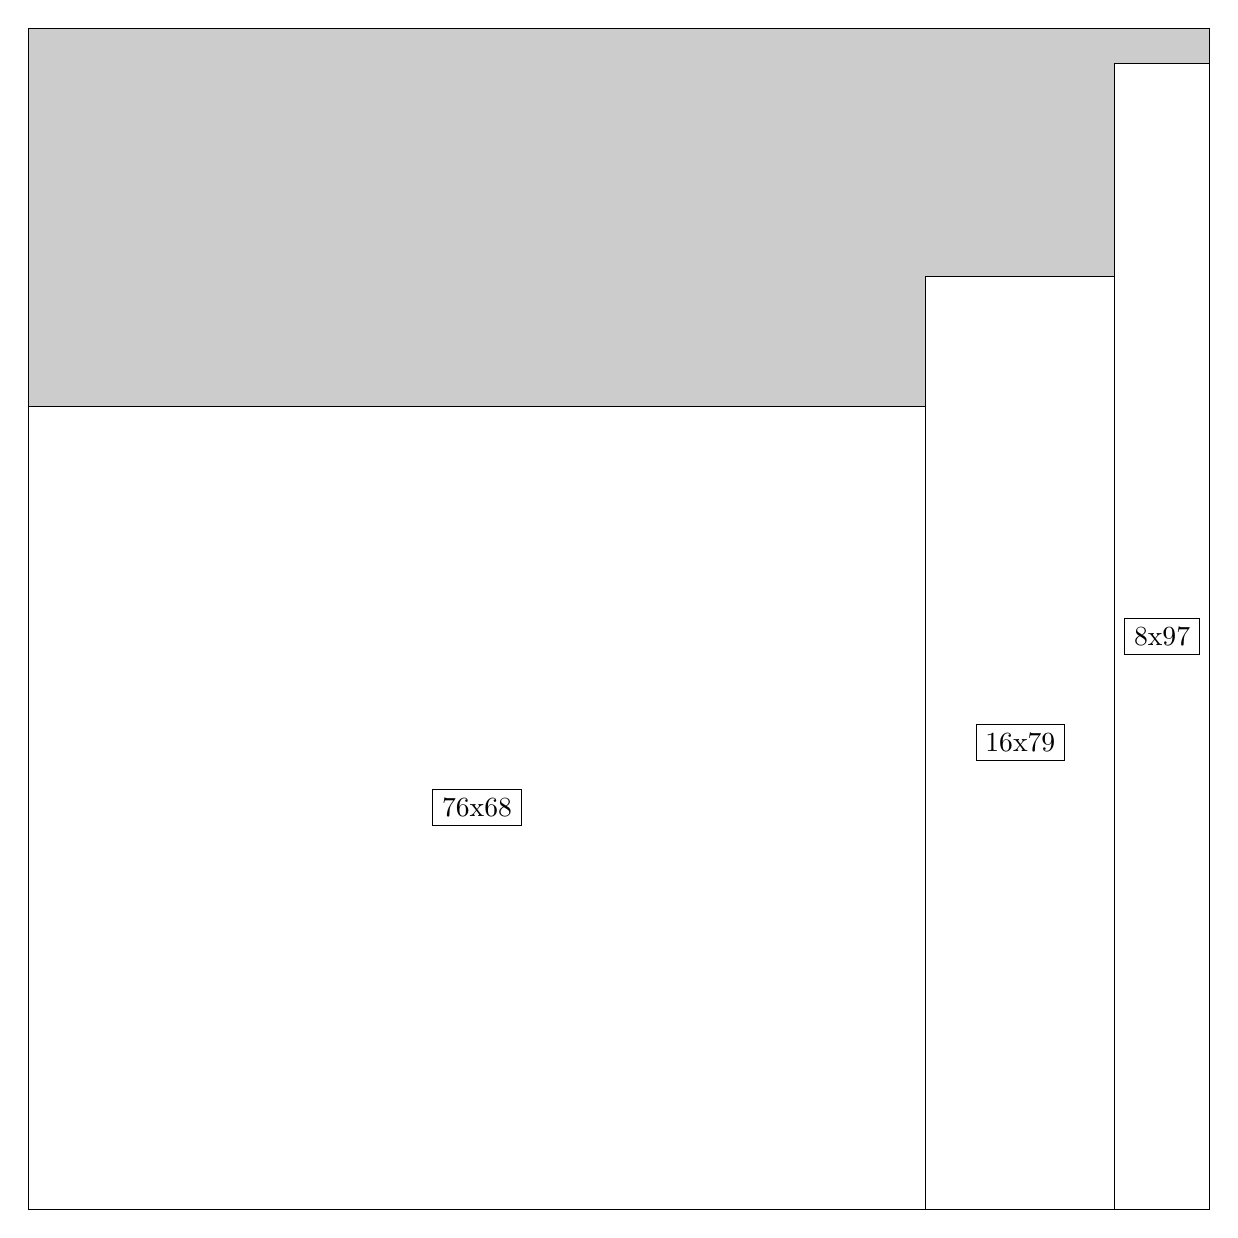
\begin{tikzpicture}[shorten >=1pt,scale=1.0,every node/.style={scale=1.0},->]
\tikzstyle{vertex}=[circle,fill=black!25,minimum size=14pt,inner sep=0pt]
\filldraw[fill=gray!40!white, draw=black] (0,0) rectangle (15.0,15.0);
\foreach \name/\x/\y/\w/\h in {76x68/0.0/0.0/11.4/10.2,16x79/11.4/0.0/2.4/11.85,8x97/13.799999999999999/0.0/1.2/14.549999999999999}
\filldraw[fill=white!40!white, draw=black] (\x,\y) rectangle node[draw] (\name) {\name} ++(\w,\h);
\end{tikzpicture}


w =76 , h =68 , x =0 , y =0 , v =5168
\par
w =16 , h =79 , x =76 , y =0 , v =1264
\par
w =8 , h =97 , x =92 , y =0 , v =776
\par
\newpage


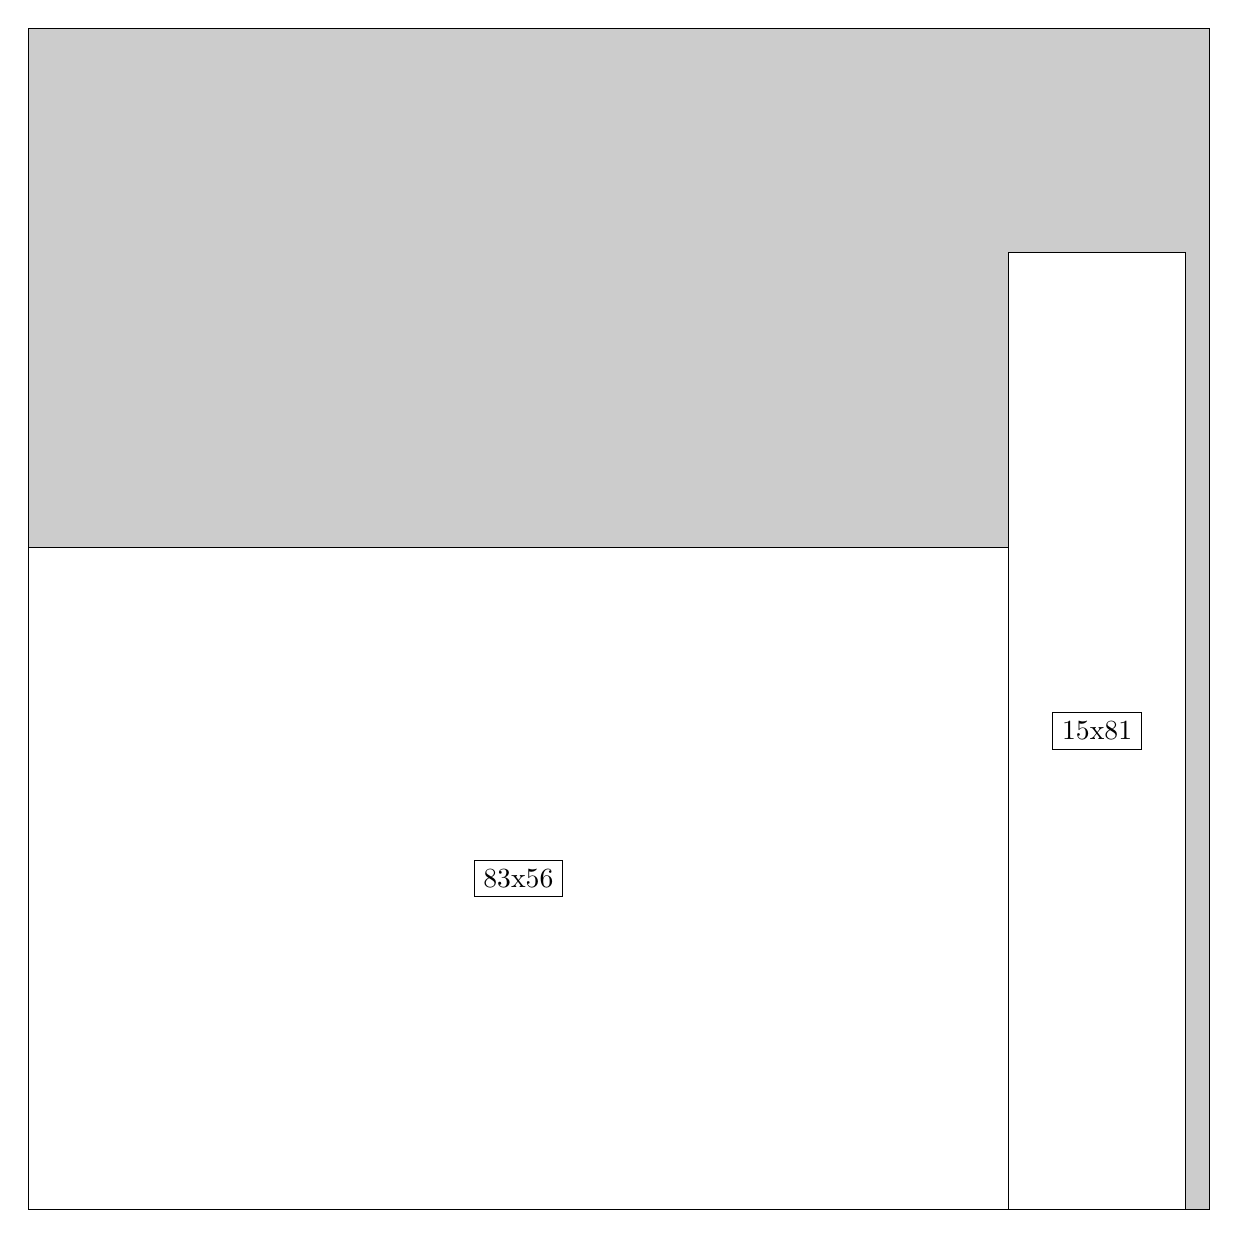
\begin{tikzpicture}[shorten >=1pt,scale=1.0,every node/.style={scale=1.0},->]
\tikzstyle{vertex}=[circle,fill=black!25,minimum size=14pt,inner sep=0pt]
\filldraw[fill=gray!40!white, draw=black] (0,0) rectangle (15.0,15.0);
\foreach \name/\x/\y/\w/\h in {83x56/0.0/0.0/12.45/8.4,15x81/12.45/0.0/2.25/12.15}
\filldraw[fill=white!40!white, draw=black] (\x,\y) rectangle node[draw] (\name) {\name} ++(\w,\h);
\end{tikzpicture}


w =83 , h =56 , x =0 , y =0 , v =4648
\par
w =15 , h =81 , x =83 , y =0 , v =1215
\par
\newpage


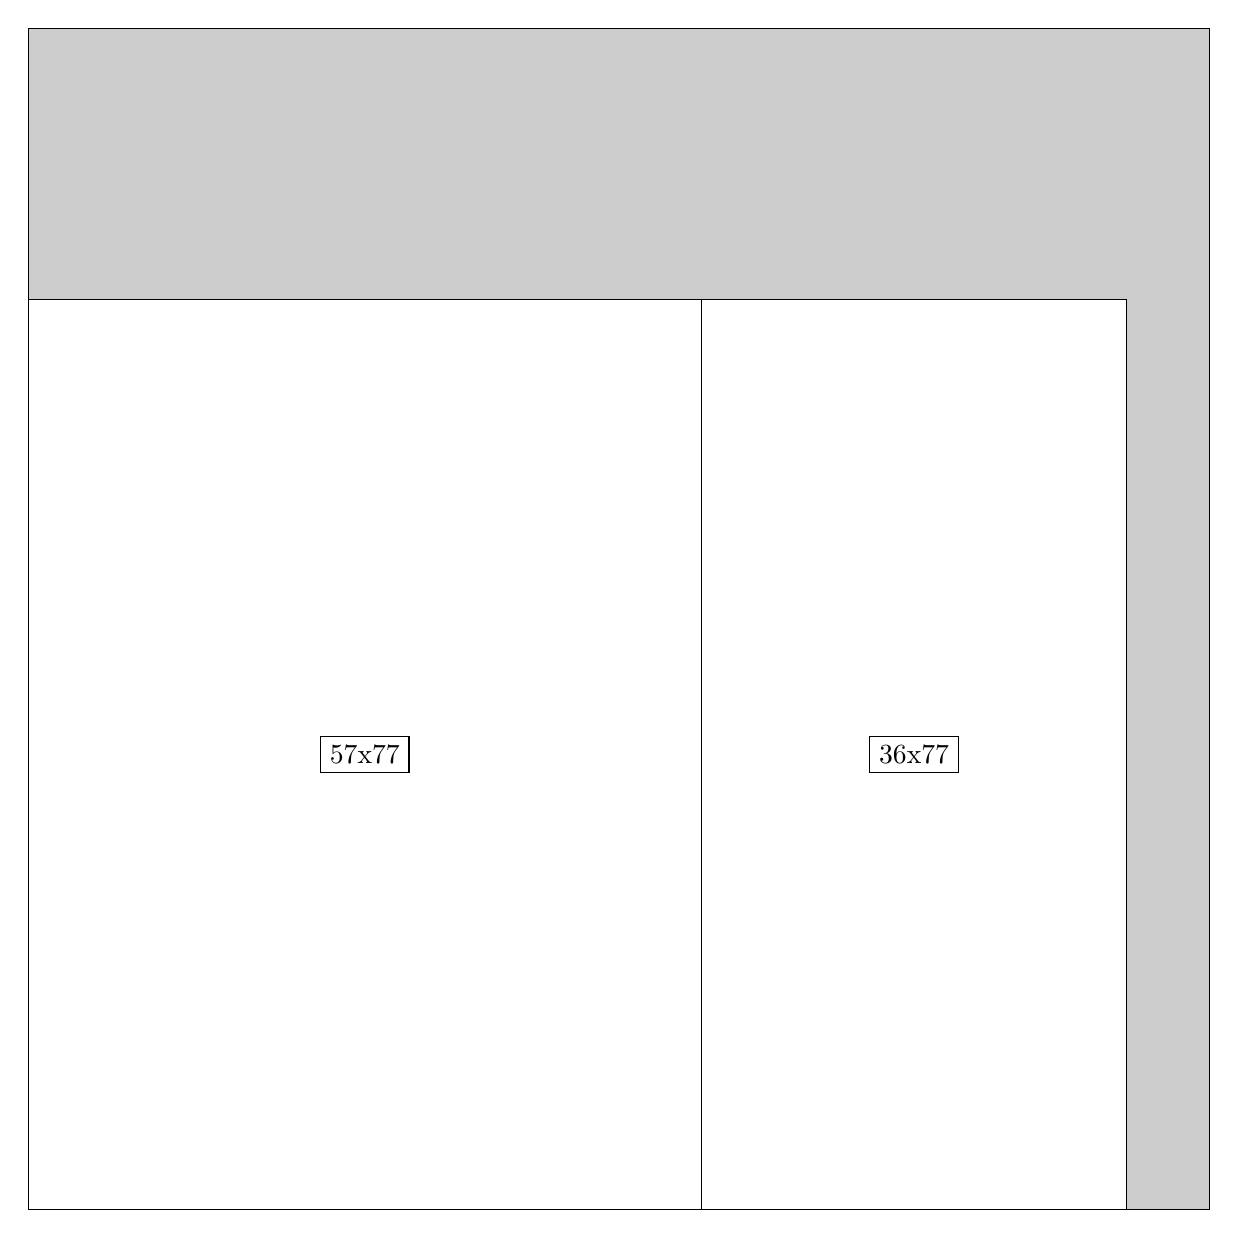
\begin{tikzpicture}[shorten >=1pt,scale=1.0,every node/.style={scale=1.0},->]
\tikzstyle{vertex}=[circle,fill=black!25,minimum size=14pt,inner sep=0pt]
\filldraw[fill=gray!40!white, draw=black] (0,0) rectangle (15.0,15.0);
\foreach \name/\x/\y/\w/\h in {57x77/0.0/0.0/8.549999999999999/11.549999999999999,36x77/8.549999999999999/0.0/5.3999999999999995/11.549999999999999}
\filldraw[fill=white!40!white, draw=black] (\x,\y) rectangle node[draw] (\name) {\name} ++(\w,\h);
\end{tikzpicture}


w =57 , h =77 , x =0 , y =0 , v =4389
\par
w =36 , h =77 , x =57 , y =0 , v =2772
\par
\newpage


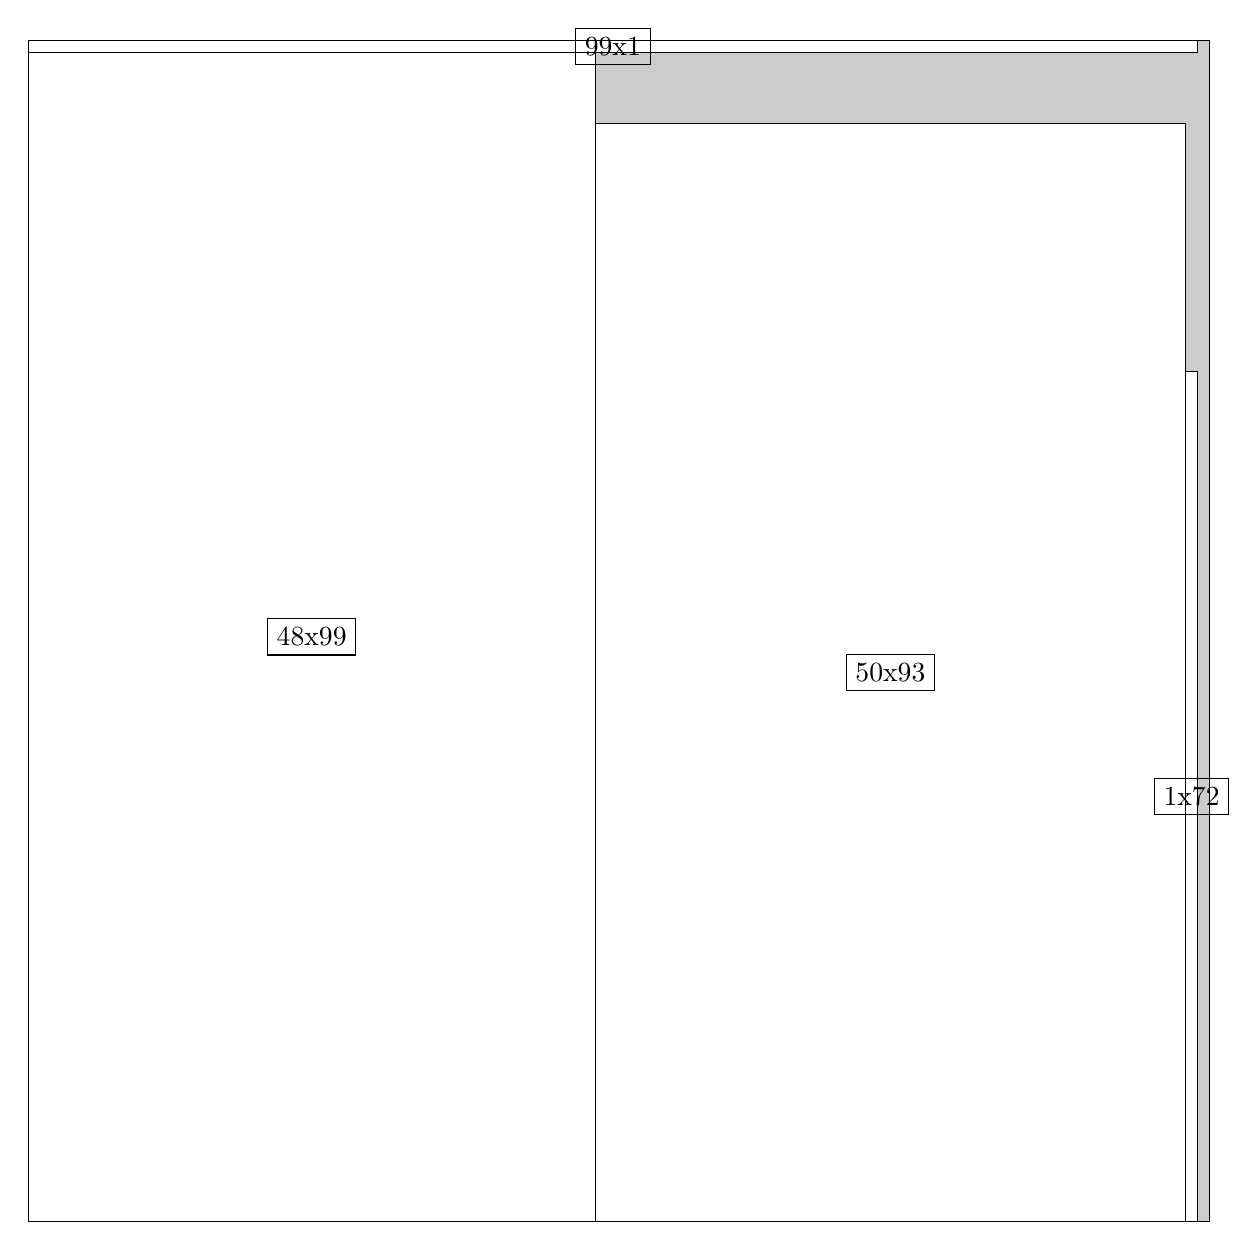
\begin{tikzpicture}[shorten >=1pt,scale=1.0,every node/.style={scale=1.0},->]
\tikzstyle{vertex}=[circle,fill=black!25,minimum size=14pt,inner sep=0pt]
\filldraw[fill=gray!40!white, draw=black] (0,0) rectangle (15.0,15.0);
\foreach \name/\x/\y/\w/\h in {48x99/0.0/0.0/7.199999999999999/14.85,50x93/7.199999999999999/0.0/7.5/13.95,99x1/0.0/14.85/14.85/0.15,1x72/14.7/0.0/0.15/10.799999999999999}
\filldraw[fill=white!40!white, draw=black] (\x,\y) rectangle node[draw] (\name) {\name} ++(\w,\h);
\end{tikzpicture}


w =48 , h =99 , x =0 , y =0 , v =4752
\par
w =50 , h =93 , x =48 , y =0 , v =4650
\par
w =99 , h =1 , x =0 , y =99 , v =99
\par
w =1 , h =72 , x =98 , y =0 , v =72
\par
\newpage


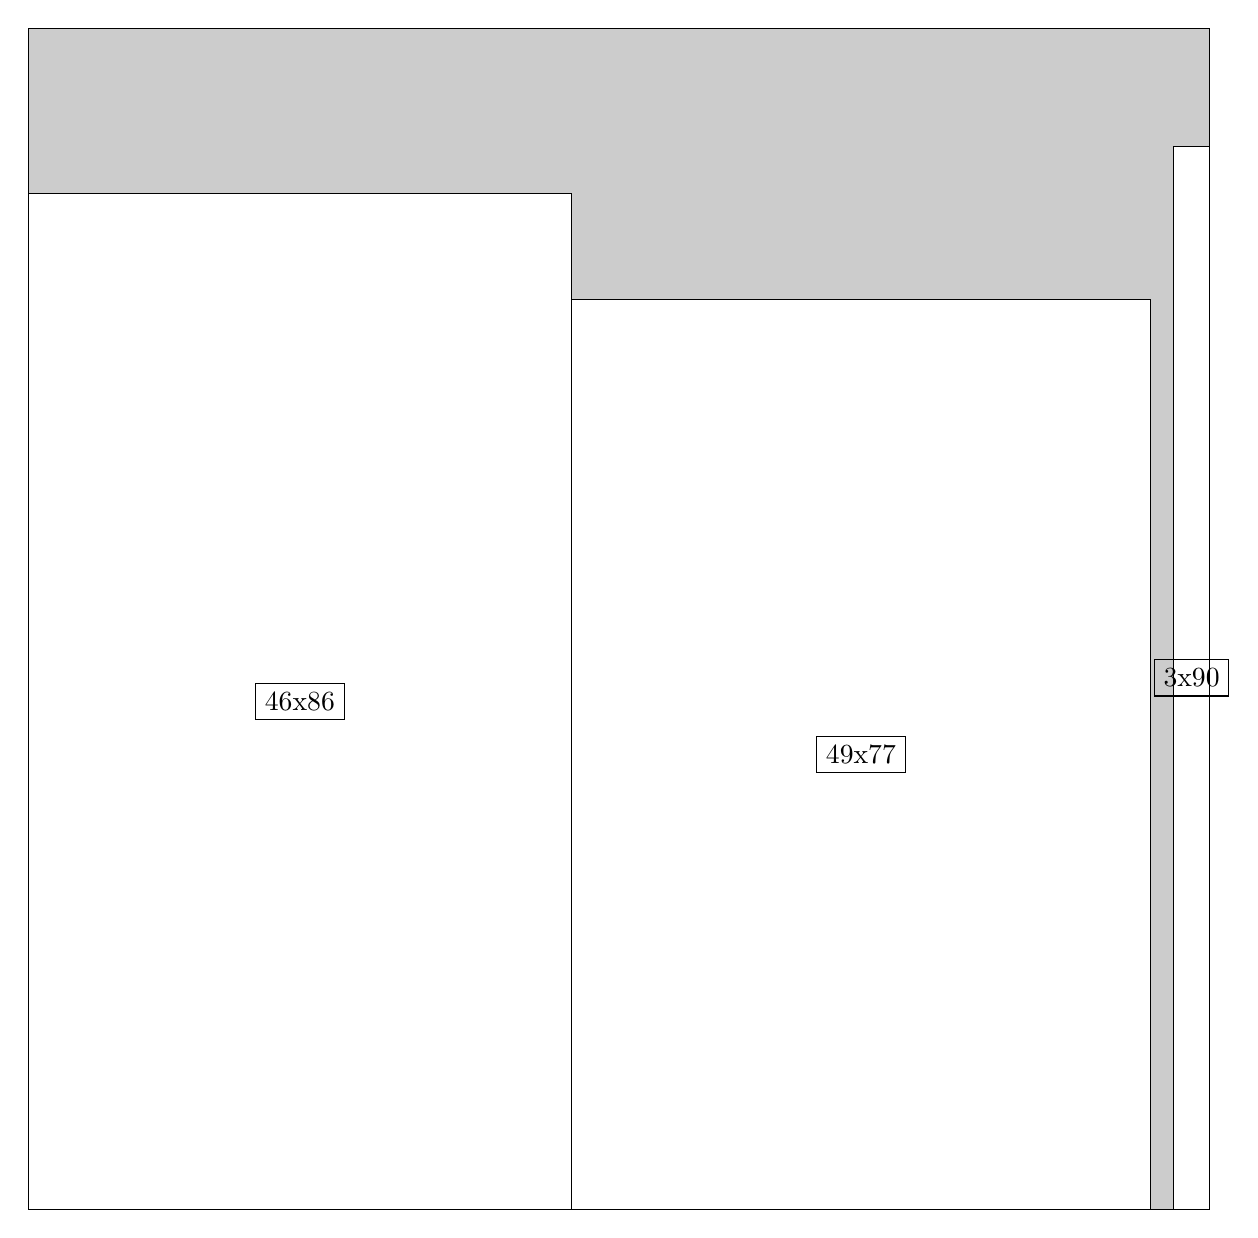
\begin{tikzpicture}[shorten >=1pt,scale=1.0,every node/.style={scale=1.0},->]
\tikzstyle{vertex}=[circle,fill=black!25,minimum size=14pt,inner sep=0pt]
\filldraw[fill=gray!40!white, draw=black] (0,0) rectangle (15.0,15.0);
\foreach \name/\x/\y/\w/\h in {46x86/0.0/0.0/6.8999999999999995/12.9,49x77/6.8999999999999995/0.0/7.35/11.549999999999999,3x90/14.549999999999999/0.0/0.44999999999999996/13.5}
\filldraw[fill=white!40!white, draw=black] (\x,\y) rectangle node[draw] (\name) {\name} ++(\w,\h);
\end{tikzpicture}


w =46 , h =86 , x =0 , y =0 , v =3956
\par
w =49 , h =77 , x =46 , y =0 , v =3773
\par
w =3 , h =90 , x =97 , y =0 , v =270
\par
\newpage


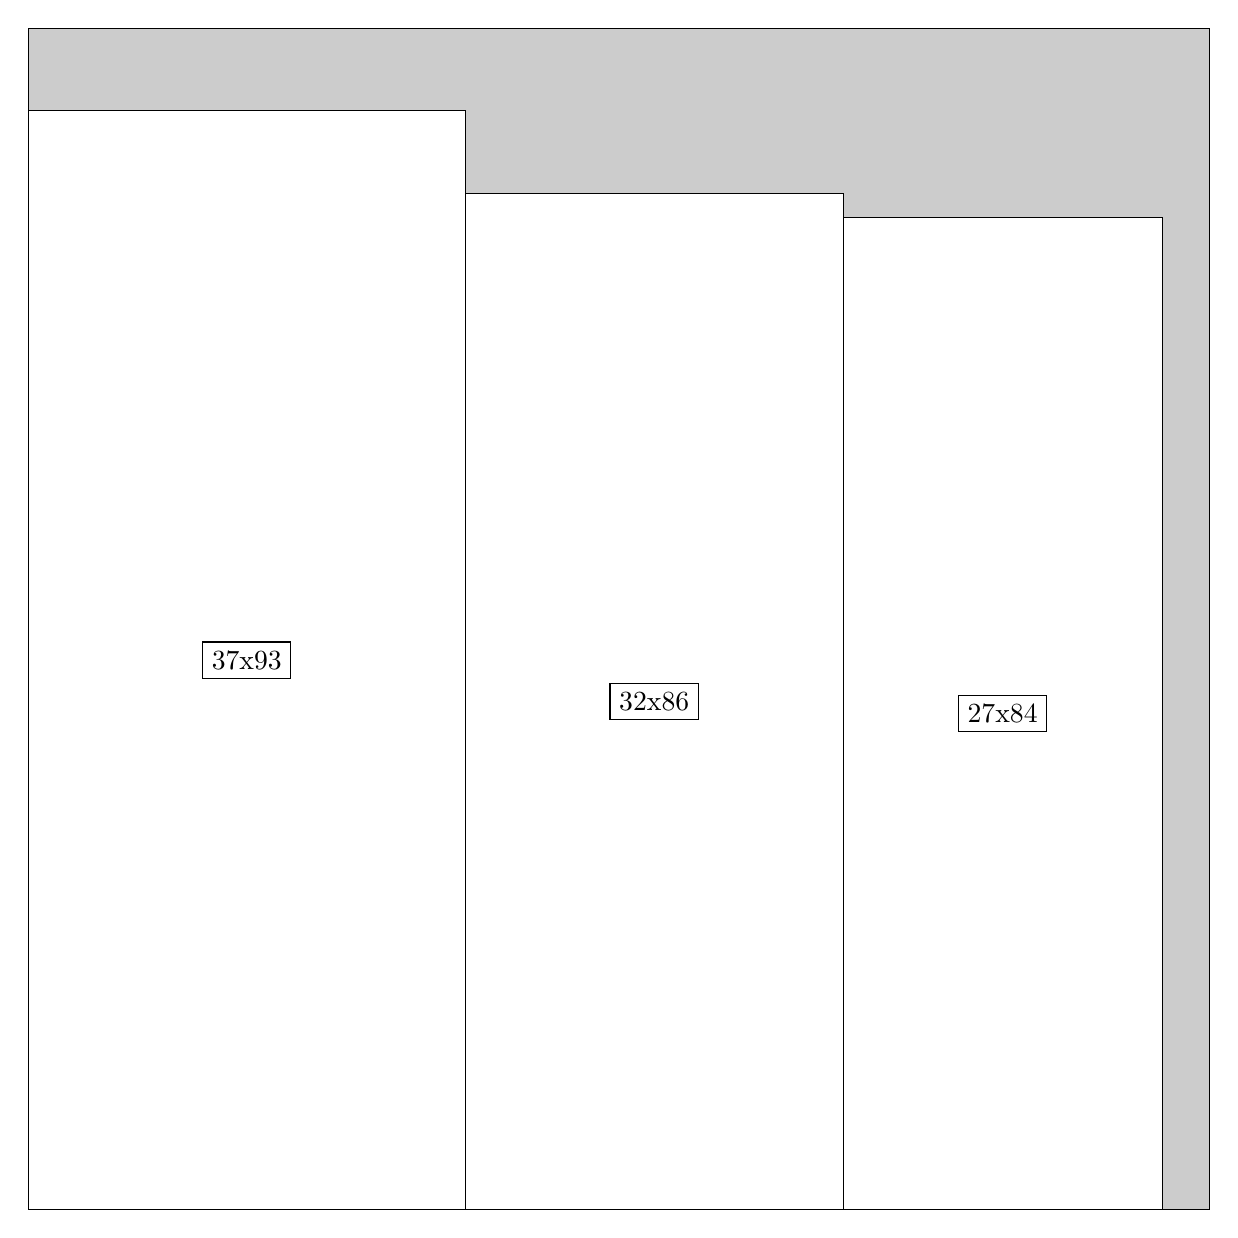
\begin{tikzpicture}[shorten >=1pt,scale=1.0,every node/.style={scale=1.0},->]
\tikzstyle{vertex}=[circle,fill=black!25,minimum size=14pt,inner sep=0pt]
\filldraw[fill=gray!40!white, draw=black] (0,0) rectangle (15.0,15.0);
\foreach \name/\x/\y/\w/\h in {37x93/0.0/0.0/5.55/13.95,32x86/5.55/0.0/4.8/12.9,27x84/10.35/0.0/4.05/12.6}
\filldraw[fill=white!40!white, draw=black] (\x,\y) rectangle node[draw] (\name) {\name} ++(\w,\h);
\end{tikzpicture}


w =37 , h =93 , x =0 , y =0 , v =3441
\par
w =32 , h =86 , x =37 , y =0 , v =2752
\par
w =27 , h =84 , x =69 , y =0 , v =2268
\par
\newpage


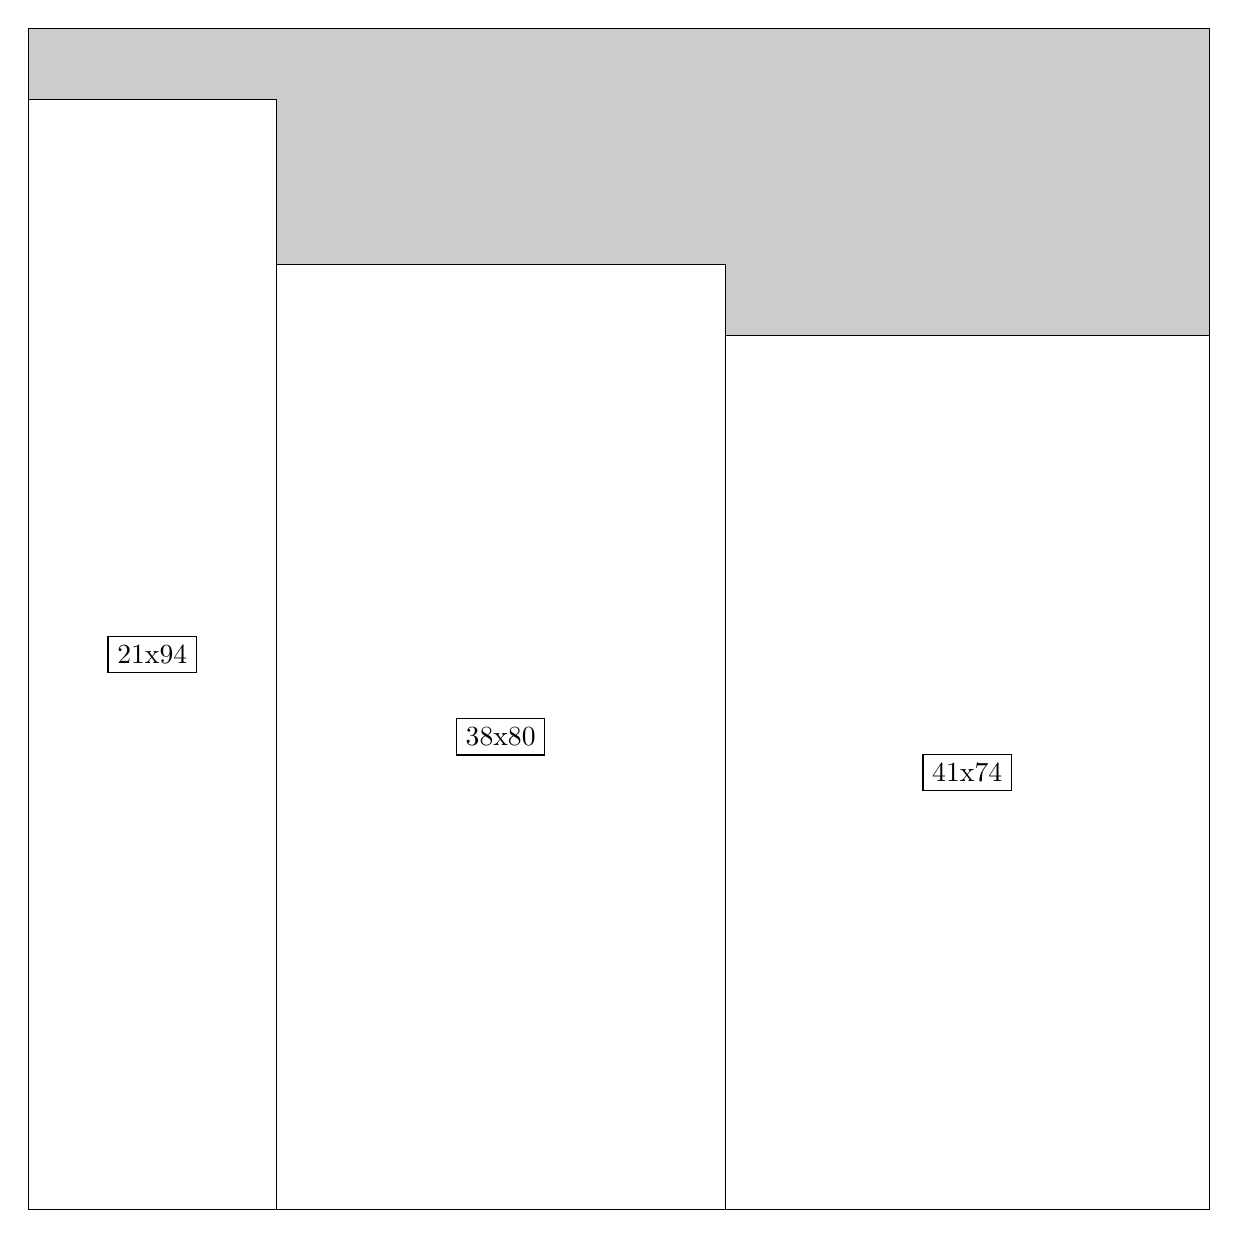
\begin{tikzpicture}[shorten >=1pt,scale=1.0,every node/.style={scale=1.0},->]
\tikzstyle{vertex}=[circle,fill=black!25,minimum size=14pt,inner sep=0pt]
\filldraw[fill=gray!40!white, draw=black] (0,0) rectangle (15.0,15.0);
\foreach \name/\x/\y/\w/\h in {38x80/3.15/0.0/5.7/12.0,41x74/8.85/0.0/6.1499999999999995/11.1,21x94/0.0/0.0/3.15/14.1}
\filldraw[fill=white!40!white, draw=black] (\x,\y) rectangle node[draw] (\name) {\name} ++(\w,\h);
\end{tikzpicture}


w =38 , h =80 , x =21 , y =0 , v =3040
\par
w =41 , h =74 , x =59 , y =0 , v =3034
\par
w =21 , h =94 , x =0 , y =0 , v =1974
\par
\newpage


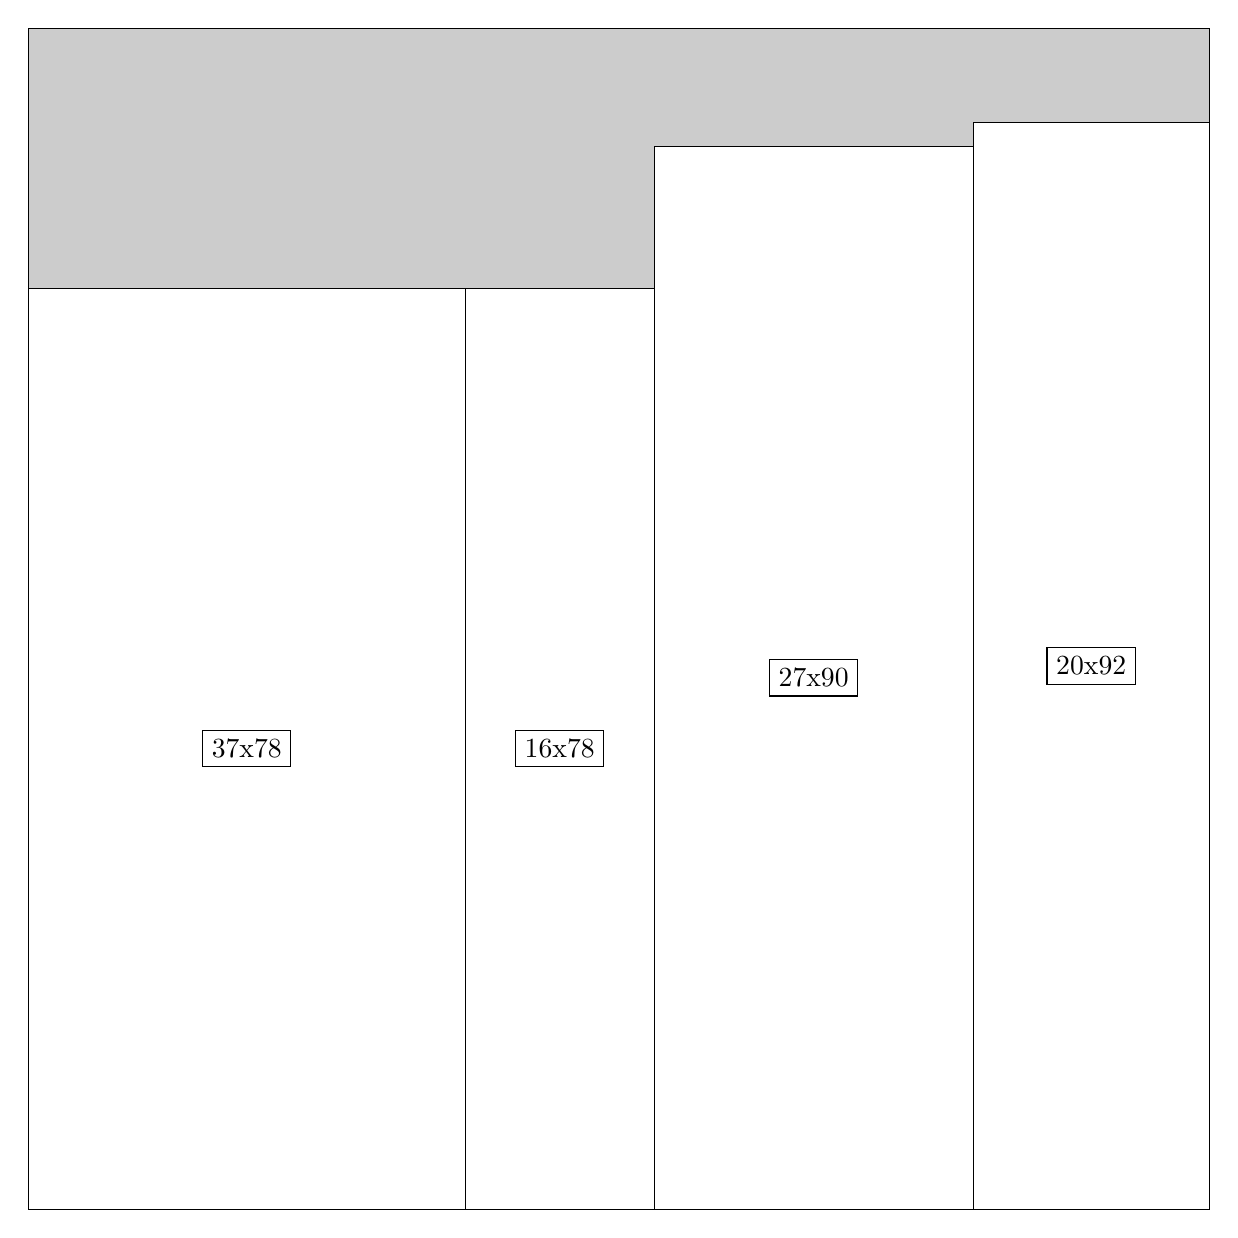
\begin{tikzpicture}[shorten >=1pt,scale=1.0,every node/.style={scale=1.0},->]
\tikzstyle{vertex}=[circle,fill=black!25,minimum size=14pt,inner sep=0pt]
\filldraw[fill=gray!40!white, draw=black] (0,0) rectangle (15.0,15.0);
\foreach \name/\x/\y/\w/\h in {37x78/0.0/0.0/5.55/11.7,27x90/7.949999999999999/0.0/4.05/13.5,20x92/12.0/0.0/3.0/13.799999999999999,16x78/5.55/0.0/2.4/11.7}
\filldraw[fill=white!40!white, draw=black] (\x,\y) rectangle node[draw] (\name) {\name} ++(\w,\h);
\end{tikzpicture}


w =37 , h =78 , x =0 , y =0 , v =2886
\par
w =27 , h =90 , x =53 , y =0 , v =2430
\par
w =20 , h =92 , x =80 , y =0 , v =1840
\par
w =16 , h =78 , x =37 , y =0 , v =1248
\par
\newpage


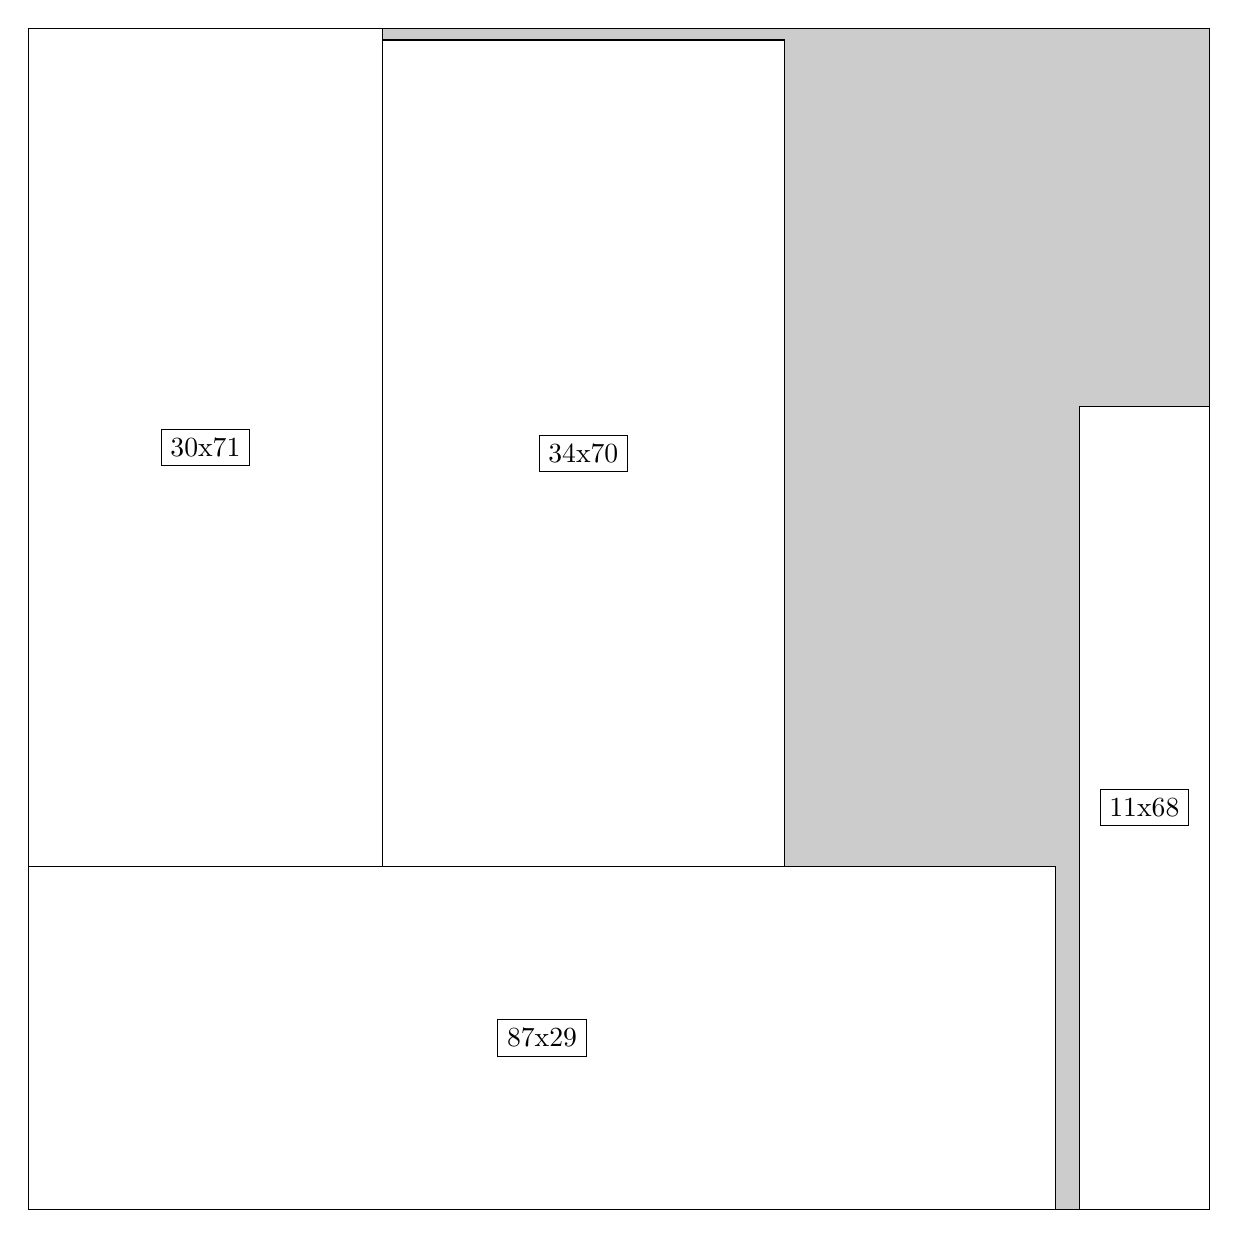
\begin{tikzpicture}[shorten >=1pt,scale=1.0,every node/.style={scale=1.0},->]
\tikzstyle{vertex}=[circle,fill=black!25,minimum size=14pt,inner sep=0pt]
\filldraw[fill=gray!40!white, draw=black] (0,0) rectangle (15.0,15.0);
\foreach \name/\x/\y/\w/\h in {87x29/0.0/0.0/13.049999999999999/4.35,34x70/4.5/4.35/5.1/10.5,30x71/0.0/4.35/4.5/10.65,11x68/13.35/0.0/1.65/10.2}
\filldraw[fill=white!40!white, draw=black] (\x,\y) rectangle node[draw] (\name) {\name} ++(\w,\h);
\end{tikzpicture}


w =87 , h =29 , x =0 , y =0 , v =2523
\par
w =34 , h =70 , x =30 , y =29 , v =2380
\par
w =30 , h =71 , x =0 , y =29 , v =2130
\par
w =11 , h =68 , x =89 , y =0 , v =748
\par
\newpage


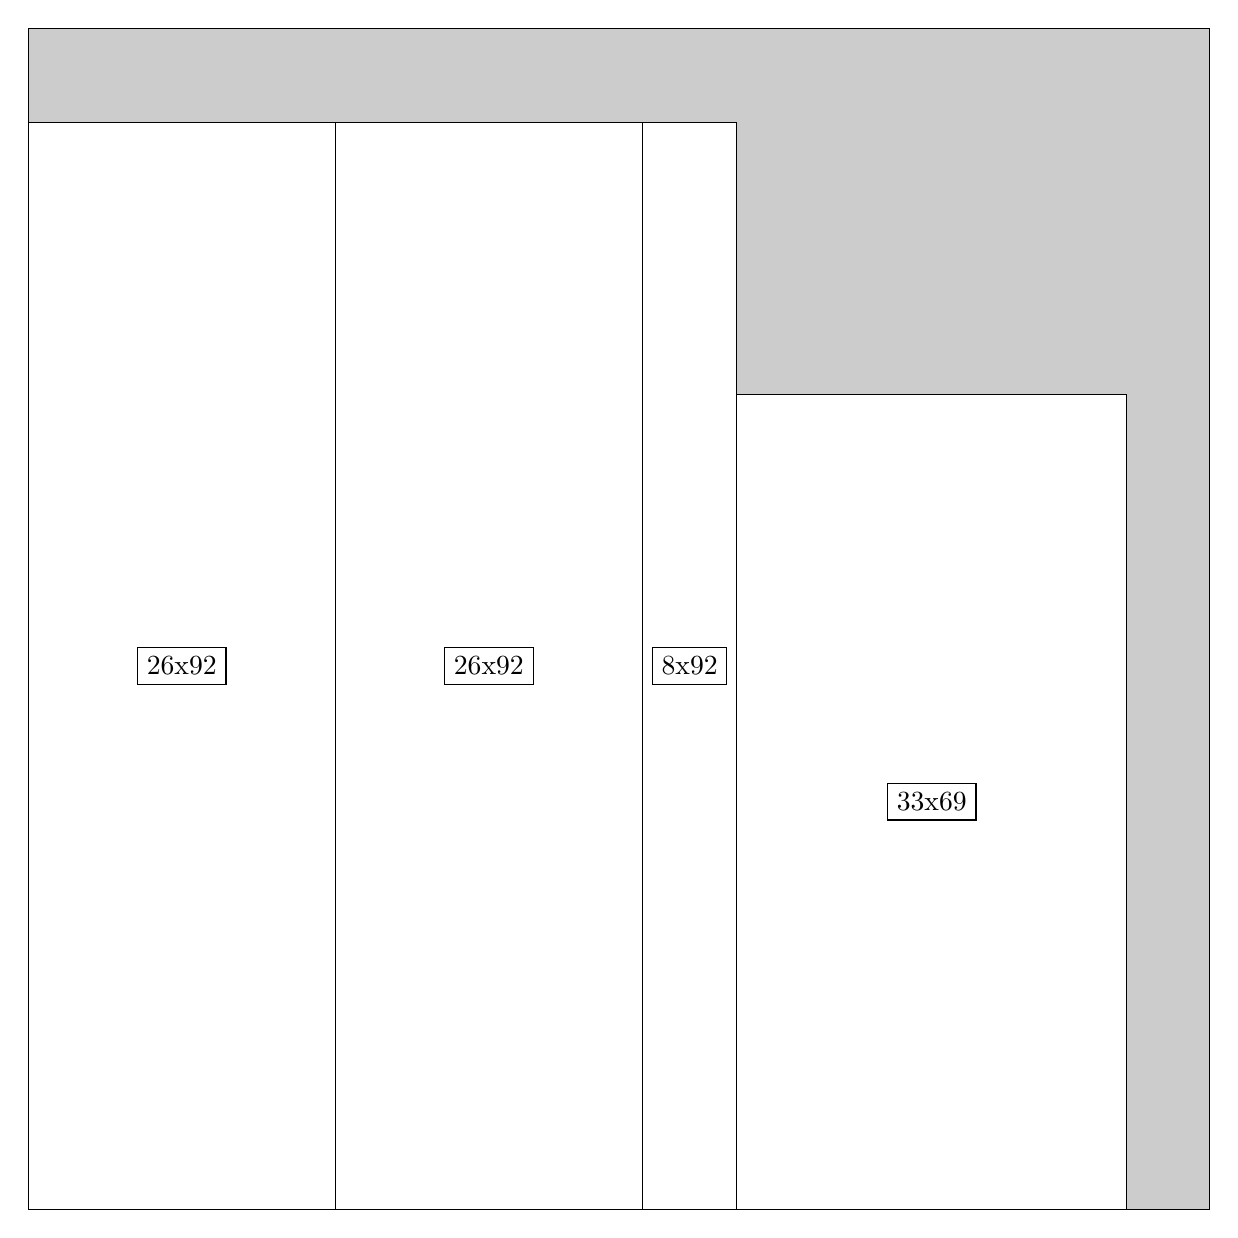
\begin{tikzpicture}[shorten >=1pt,scale=1.0,every node/.style={scale=1.0},->]
\tikzstyle{vertex}=[circle,fill=black!25,minimum size=14pt,inner sep=0pt]
\filldraw[fill=gray!40!white, draw=black] (0,0) rectangle (15.0,15.0);
\foreach \name/\x/\y/\w/\h in {26x92/0.0/0.0/3.9/13.799999999999999,26x92/3.9/0.0/3.9/13.799999999999999,33x69/9.0/0.0/4.95/10.35,8x92/7.8/0.0/1.2/13.799999999999999}
\filldraw[fill=white!40!white, draw=black] (\x,\y) rectangle node[draw] (\name) {\name} ++(\w,\h);
\end{tikzpicture}


w =26 , h =92 , x =0 , y =0 , v =2392
\par
w =26 , h =92 , x =26 , y =0 , v =2392
\par
w =33 , h =69 , x =60 , y =0 , v =2277
\par
w =8 , h =92 , x =52 , y =0 , v =736
\par
\newpage


\end{document}